% The rewriting relation \( \Rightarrow_{\mathcal{A},\mathfrak{M}} \) is terminating relative to $\Rightarrow_{\mathcal{B},\mathfrak{M}}$ if the following hold: (i) for all \(G \Rightarrow_{\mathcal{A},\mathfrak{M}} H\), \( w_{s_\mathbb{X}}(G) > w_{s_\mathbb{X}}(H) \), and (ii) for all \(G \Rightarrow_{\mathcal{B},\mathfrak{M}} H\), \( w_{s_\mathbb{X}}(G) \geq w_{s_\mathbb{X}}(H) \). However, directly verifying all rewriting steps is infeasible due to their potential infiniteness. 
% Thus, we aim to provide a rule-based sufficient condition for termination.
% \begin{remark}

\begin{notation}
    % \noindent
    % \begin{minipage}{0.6\textwidth}\setlength{\parindent}{1em}
     Let \( \mathcal{X}\) be a ruler-graph with underlying graph $X$. Let \( A, B, G \) be graphs. Let \( \alpha \colon A \to G \) and \( \beta \colon B \to G \) be morphisms. 
    We define the following sets of monomorphisms of $X$ in $G$: 
        %  the set $\operatorname{Mono}(X,G,\alpha)$ of occurrences which is fully included in $A$; the set $\operatorname{Mono}(X,G,\lnot \alpha)$ of occurrences which is not fully included in $A$; the set $\operatorname{Mono}(X,G,\lnot \alpha, \beta)$ of occurrences which is not fully included in $A$ but fully includedin $B$; the set $\operatorname{Mono}(X,G,\lnot \alpha, \lnot \beta)$ of occurrences which is neither fully included in $A$ nor fully includedin $B$. Formally:
    % \end{minipage}%
    % \begin{minipage}{0.38\textwidth}
    %     \hfill
    %     \begin{tikzpicture}[scale=0.9]
    %         \node (X) at (-0.5,0) {$X$};
    %         \node (G) at (1,0) {$G$}; 
    %         \node (A) at (3,0.2) {$A$}; 
    %         \node (B) at (3,-0.2) {$B$}; 
    %         \draw [>->] (X) to (G);
    %         \draw [>->] (A) to node [above,label,pos=0.5] {$\alpha$} (G);
    %         \draw [>->] (B) to node [below,label,pos=0.5] {$\beta$} (G);
    %     \end{tikzpicture}
    % \end{minipage}%
    \begin{align*}
        \operatorname{Mono}(\mathcal{X},G,\alpha) &= \left\{ \iota \colon X \rightarrowtail G \;\middle|\; \exists \beta \colon X \rightarrowtail A.\, \iota = \beta \star \alpha \right\}, 
        \\
        \operatorname{Mono}(\mathcal{X},G,\lnot \alpha) &= \left\{ \iota \colon X \rightarrowtail G \;\middle|\; \nexists \beta \colon X \rightarrowtail A.\, \iota = \beta \star \alpha \right\}, 
        \\
        \operatorname{Mono}(\mathcal{X},G,\lnot \alpha, \beta) &= \left\{ 
            \iota \colon X \rightarrowtail G \;\middle|\; 
                \begin{aligned}  
                    &(\nexists \zeta \colon X \rightarrowtail A.\, \iota = \zeta \star \alpha) \\ 
                    &\land (\exists \zeta \colon X \rightarrowtail B.\, \iota = \zeta \star \beta)
                \end{aligned}
        \right\},
        \\
        \operatorname{Mono}(\mathcal{X},G,\lnot \alpha, \lnot \beta) &= \left\{ 
            \iota \colon X \rightarrowtail G \;\middle|\; 
                \begin{aligned}
                    &(\nexists \zeta \colon X \rightarrowtail A.\, \iota = \zeta \star \alpha) \\
                    &\land (\nexists \zeta \colon X \rightarrowtail B.\, \iota = \zeta \star \beta)
                \end{aligned}
        \right\}.
    \end{align*}
    For a set $\operatorname{Mono}(\mathcal{X},\dots)$, we define $\operatorname{Mono}(\mathcal{X},\dots)_{\operatorname{NF}}$ as the subset of \( X \)-occurrences that are not included in any occurrence of its forbidden context if exists, and  $\operatorname{Mono}(\mathcal{X},\dots)_{\operatorname{F}}$ as the subset of \( X \)-occurrences that are included in some occurrences of its forbidden context if exists.
\end{notation}

% \trackedtext{
%     \begin{itemize}
%         % \item explicit $X$-occurrences in $L$ or $R$ that are included in some occurrences of its forbidden context in $L$ or $R$: we do not need to consider these $X$-occurrences
%         \item explicit $X$-occurrences in implicit $F$-occurrences: \\
%          explicit $X$-occurrences in $L$ or $R$ that are not included in some occurrences of its forbidden context in $L$ or $R$
%             \begin{itemize}
%                 \item These $X$-occurrences may be included in some occurrences of its forbidden context 
%             \end{itemize}
%         \item implicit $X$-occurrences in implicit $F$-occurrences : \\
%             \begin{itemize}
%                 \item $\rho$ should be $X$-non increasing : all elements in $D(R,X)$ has corresponding subgraphs with the same interface elements in $D(L,X)$
%                 \item $\rho^{-1}$ should be $F$-non increasing: all elements in $D(L,F)$ has corresponding subgraphs with the same interface elements in $D(R,F)$
%                 \item 
%             \end{itemize}
%         \item implicit $X$-occurrences in explicit $F$-occurrences
%     \end{itemize}
% }
% \textcolor{blue}{
% \begin{definition}
%     \label{def:predictable}
%     Let $\mathcal{X}$ be a ruler-graph with underlying graph $X$ and let \( \rho = (L \overset{l}{\leftarrowtail} K \overset{r}{\rightarrowtail} R) \) be a rule. 
%     Let \( M_X: \operatorname{Mono}(\mathcal{X}, L)_F \to \operatorname{Mono}(\mathcal{X}, R)_F \) and $M_F: \operatorname{Mono}(F,L) \rightarrow \operatorname{Mono}(F,R)$ be injections and $\Psi$ be a function associating $L' \in D(L,F)$ to a homomorphism in $\operatorname{Mono}(L',R)$. 
%     We say that \textbf{the number of $X$-occurrences that are not included in any occurrences of its forbidden context in any $\rho$-rewriting step is predictable relative to $(M_X,M_F,\Psi)$} if either $\mathcal{X} = (X)$ and $\rho$ is $X$-non-increasing,
%     or $\mathcal{X} = (X,f:X \rightarrowtail F)$ the following conditions hold:
%     \begin{enumerate} 
%         \item \label{hyp:rho_x_non_increasing}
%         % The number of occurrences of $X$ is non-increasing from left to right in a rewriting step using $\rho^{-1}$ or $\rho$.
%                 $\rho$ is $X$-non-increasing, \todo{used in~\autoref{lem:xglnotmlnotlp_xhlnotmrnotrp}}
%         \item \label{hyp:rho_rev_x_non_increasing} $\rho^{-1}$ is $X$-non-increasing, \todo{used in~\autoref{lem:xglnotmlnotlp_xhlnotmrnotrp}}
%         \item \label{hyp:f_non_increasing}
%         % The number of occurrences of $F$ is non-increasing from left to right in a rewriting step using $\rho^{-1}$ under $\Psi$.
%         $\rho^{-1}$ is $F$-non-increasing under $\Psi$, \todo{used in~\autoref{lem:xglnotmlp_xhlnotmrp}}
%         \item \label{hyp:inj_mono_x_l_to_r}
%         for every \( h_{XL} \in \operatorname{Mono}(\mathcal{X}, L)_F \),  we can construct the diagram below (intuitively, the images of $h_{XL}$ and $M_X(h_{XL})$ share the same interface elements):
%         \begin{center}
%             \resizebox{0.3\textwidth}{!}{
%                 \begin{tikzpicture}
%                     \node (k) {K}; 
%                     \node (k') [above=of k] {$K'$};
%                     \node (l) [left=of k] {$L$};
%                     \node (rb) [above=of l] {$X$};
%                     \node (r) [right=of k] {$R$};
%                     \node (rb') [above=of r] {$X$};
%                     \draw[<-<]  (l) -- (k) node [midway,above] {l};
%                     \draw[<-<]  (r) -- (k) node [midway,above] {r};
%                     \draw[>->]  (k') -- (rb') node [midway,above] {};
%                     \draw[>->]  (rb') -- (r) node [midway,right] {$M_X(h_{XL})$};
%                     \draw[>->]  (k') -- (rb) node [midway, right] {};
%                     \draw[>->]  (k') -- (k);
%                     \draw[>->]  (rb) -- (l) node [midway,below] {};
%                     \node () [at=($(k)!0.5!(rb)$)] {PB};
%                     \node () [at=($(k)!0.5!(rb')$)] {PB};
%                 \end{tikzpicture}
%             }
%         \end{center}
%         \todo{where do we need this assumption?}
%         \item \label{hyp:inj_mono_f_l_to_r} for every $h_{FL} \in \operatorname{Mono}(F,L)$, we can construct the diagram below (intuitively, the images of $h_{FL}$ and $M_F(h_{FL})$ have the same interface elements):
%             \begin{center}
%                 \resizebox{0.3\textwidth}{!}{
%                     \begin{tikzpicture}
%                         \node (k) {K}; 
%                         \node (k') [above=of k] {$K'$};
%                         \node (l) [left=of k] {$L$};
%                         \node (rb) [above=of l] {$F$};
%                         \node (r) [right=of k] {$R$};
%                         \node (rb') [above=of r] {$F$};
%                         \draw[<-<]  (l) -- (k) node [midway,above] {l};
%                         \draw[<-<]  (r) -- (k) node [midway,above] {r};
%                         \draw[>->]  (k') -- (rb') node [midway,above] {};
%                         \draw[>->]  (rb') -- (r) node [midway,right] {$M_F(h_{FL})$};
%                         \draw[>->]  (k') -- (rb) node [midway, right] {};
%                         \draw[>->]  (k') -- (k);
%                         \draw[>->]  (rb) -- (l) node [midway,below] {};
%                         \node () [at=($(k)!0.5!(rb)$)] {PB};
%                         \node () [at=($(k)!0.5!(rb')$)] {PB};
%                     \end{tikzpicture}
%                 }
%             \end{center} 
%             \item \label{hyp:inj_mono_f_l_to_r_} for every $h_{FL} \in \operatorname{Mono}(F,L)$, for every \( h_{XL} \in \operatorname{Mono}(\mathcal{X}, L)_F \), if $h_{XL} = h_{XF} \star h_{FL}$ then $M_X(h_{XL}) = h_{XF} \star M_F(h_{FL})$.
%              \todo{where do we need this assumption?}
%         \item \label{hyp:f_implicitly_destroyed} for every $L' \in D(L,F)$ and every $h_{XL'}:X \rightarrowtail L'$, \todo{problem!! we can not apply $M_X$} we have $M_X(h_{XL'} \star h_{L'L}) = h_{XL'} \star \Psi(L')$ where $h_{L'L}$ is the inclusion function from $L'$ to $L$.
%          \todo{where do we need this assumption?}
%     \end{enumerate}
% \end{definition}
% }
% \trackedtext{Intuitively, the first condition ensures in every rewriting step using $\rho$, there are as many implicit $X$-occurrences in $H$ as in $G$.
% \\
% The second condition ensures that for every implicit $F$-occurrence in $G$, there is a corresponding implicit $F$-occurrence in $H$ with the same interface elements.
% \\
% The third condition ensures that every $X$-occurrence that is included in an $X$-occurrence in $L$ is mapped to an $X$-occurrence in $R$ with the same interface elements by $M_X$. 
% \\
% % The third condition ensures that every explicit $X$-occurrence that is included in an explicit $X$-occurrence in $G$ is mapped to an explicit $X$-occurrence in $H$ with the same interface elements by $M_X$. 
% The fourth condition ensures that every $F$-occurrence in $L$ is mapped to an $F$-occurrence in $R$ with the same interface elements by $M_F$.
% \\
% The fifth condition ensures that for every $X$-occurrence that is included in an $F$-occurrence in $L$, the corresponding $X$-occurrence in $R$ by $M_X$ is also included in an $F$-occurrence in $R$ by $M_F$.
% \\
% The last condition ensures that every $X$-occurrence that is included in a subgraph $L'$ of $L$ that can form an occurrence of $F$ with a subgraph of the context graph is mapped to a distinguished subgraph of $R$ by $\Psi$, and the mapping preserves the implicit $X$-occurrences.
% }


\noindent
\begin{minipage}{0.7\textwidth}\setlength{\parindent}{1em}
    Let $\mathcal{X}$ be a ruler-graph with underlying graph $X$ and \( \rho = (L \overset{l}{\leftarrowtail} K \overset{r}{\rightarrowtail} R) \) be a rule. 
    Suppose that $\rho^{-1}$ is $F$-non-increasing if $\mathcal{X}= (X,f:X \rightarrowtail F)$ and, $\rho$ and $\rho^{-1}$ are $X$-non-increasing.
    % Suppose that the number of $X$-occurrences that are not included in any occurrences of the forbidden context in a $\rho$-rewriting step is predictable (\autoref{def:predictable}). 
    Consider the DPO diagram illustrated on the right. 
\end{minipage}%
\begin{minipage}{0.29\textwidth}
    \hfill
    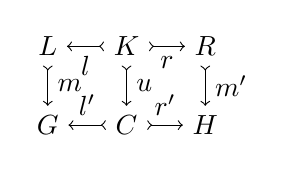
\begin{tikzpicture}
        % [node distance=15mm]
        \node (I) {$K$};
        \node (L) [left of=I] {$L$};
        \node (R) [right of=I] {$R$};
        \node (G) [below of=L] {$G$};
        \node (C) [below of=I] {$C$};
        \node (H) [below of=R] {$H$}; 
        \draw [>->] (I) to  node [midway,below] {$l$} (L);
        \draw [>->] (I) to  node [midway,below] {$r$} (R);
        \draw [>->] (L) to node [midway,right] {$m$} (G);
        \draw [>->] (I) to  node [midway,right] {$u$} (C); 
        \draw [>->] (R) to  node [midway,right] {$m'$} (H);
        \draw [>->] (C) to node [midway,above] {$l'$} (G);
        \draw [>->] (C) to node [midway,above] {$r'$} (H);
        % \node [at=($(I)!.5!(G)$)] {\normalfont PO};
        % \node [at=($(I)!.5!(H)$)] {\normalfont PO};
      \end{tikzpicture}
\end{minipage} 

\vspace{1mm}
% The following decompositions hold:
% \begin{flalign*}
%     \operatorname{Mono}(\mathcal{X},G)_{\operatorname{NF}} &= 
%     \operatorname{Mono}(\mathcal{X},G,m)_{\operatorname{NF}}
%     \uplus
%     \operatorname{Mono}(\mathcal{X},G,\lnot m, l')_{\operatorname{NF}} 
%     \uplus
%     \operatorname{Mono}(\mathcal{X},G,\lnot m, \lnot l')_{\operatorname{NF}}
%     \\
%     \operatorname{Mono}(\mathcal{X},H)_{\operatorname{NF}} &= 
%     \operatorname{Mono}(\mathcal{X},H,m')_{\operatorname{NF}}
%     \uplus
%     \operatorname{Mono}(\mathcal{X},H,\lnot m', r')_{\operatorname{NF}}
%     \uplus
%     \operatorname{Mono}(\mathcal{X},H,\lnot m', \lnot r')_{\operatorname{NF}}
% \end{flalign*}

The set $\operatorname{Mono}(\mathcal{X},G)_{\operatorname{NF}}$ can be partitioned into three disjoint sets:
$$
    \operatorname{Mono}(\mathcal{X},G,m)_{\operatorname{NF}}
    \uplus
    \operatorname{Mono}(\mathcal{X},G,\lnot m, l')_{\operatorname{NF}} 
    \uplus
    \operatorname{Mono}(\mathcal{X},G,\lnot m, \lnot l')_{\operatorname{NF}}
$$
and $\operatorname{Mono}(\mathcal{X},H)_{\operatorname{NF}}$ can be partitioned into three disjoint sets:
$$
\operatorname{Mono}(\mathcal{X},H,m')_{\operatorname{NF}}
    \uplus
    \operatorname{Mono}(\mathcal{X},H,\lnot m', r')_{\operatorname{NF}}
    \uplus
    \operatorname{Mono}(\mathcal{X},H,\lnot m', \lnot r')_{\operatorname{NF}}
$$
Thus, we have 
\begin{flalign*}
    &\card{\operatorname{Mono}(\mathcal{X},G)_{\operatorname{NF}}} - 
    \card{\operatorname{Mono}(\mathcal{X},H)_{\operatorname{NF}}} 
    \\=
    &(\card{\operatorname{Mono}(\mathcal{X},G,m)_{\operatorname{NF}}} 
        -  
    \card{\operatorname{Mono}(\mathcal{X},H,m')_{\operatorname{NF}}}) 
    + 
    \\
    &(
        \card{\operatorname{Mono}(\mathcal{X},G,\lnot m, l')_{\operatorname{NF}}}
             - 
        \card{\operatorname{Mono}(\mathcal{X},H,\lnot m', r')_{\operatorname{NF}}}) + \\
    &(
        \card{\operatorname{Mono}(\mathcal{X},G,\lnot m, \lnot l')_{\operatorname{NF}}} 
            - 
        \card{\operatorname{Mono}(\mathcal{X},H,\lnot m', \lnot r')_{\operatorname{NF}}}
    )
\end{flalign*}
To estimate $\card{\operatorname{Mono}(\mathcal{X},G)_{\operatorname{NF}}} - 
    \card{\operatorname{Mono}(\mathcal{X},H)_{\operatorname{NF}}}$, we establish the following lemmas.
% The following lemmas can be used to approximate $\card{\operatorname{Mono}(\mathcal{X},G)_{\operatorname{NF}}} - 
%     \card{\operatorname{Mono}(\mathcal{X},H)_{\operatorname{NF}}}$
\begin{lemma}
    \label{lem:xglnotmlp_xhlnotmrp}
        Let $\mathcal{X}$ be a ruler-graph with underlying graph $X$ and \( \rho = (L \overset{l}{\leftarrowtail} K \overset{r}{\rightarrowtail} R) \) be a rule. 
        Suppose that $\rho^{-1}$ is $F$-non-increasing if $\mathcal{X} = (X,f:X \rightarrowtail F)$.
        We have 
    $$\card{\operatorname{Mono}(\mathcal{X},G,\lnot m, l')_{\operatorname{NF}}} \geq
        \card{\operatorname{Mono}(\mathcal{X},H,\lnot m', r')_{\operatorname{NF}}}$$
\end{lemma} 
\begin{proof} 
    See~\textsection~\ref{antipattern:proof:lem:xglnotmlp_xhlnotmrp}.
 \end{proof}
\begin{lemma}
    \label{lem:xglnotmlnotlp_xhlnotmrnotrp}
        Let $\mathcal{X}$ be a ruler-graph with underlying graph $X$ and \( \rho = (L \overset{l}{\leftarrowtail} K \overset{r}{\rightarrowtail} R) \) be a rule. Suppose that $\rho$ and $\rho^{-1}$ are $X$-non-increasing. We have
    $$ 
        \card{\operatorname{Mono}(\mathcal{X},G,\lnot m, \lnot l')_{\operatorname{NF}}} \geq
        \card{\operatorname{Mono}(\mathcal{X},H,\lnot m', \lnot r')_{\operatorname{NF}}}
    $$
\end{lemma}
\begin{proof}
    See~\textsection~\ref{antipattern:proof:lem:xglnotmlnotlp_xhlnotmrnotrp}.
 \end{proof}

The following inequality follows.
 \begin{flalign*}
     \card{\operatorname{Mono}(\mathcal{X},G)_{\operatorname{NF}}} - 
     \card{\operatorname{Mono}(\mathcal{X},H)_{\operatorname{NF}}} 
     \geq
     \card{\operatorname{Mono}(\mathcal{X},G,m)_{\operatorname{NF}}} - \card{\operatorname{Mono}(\mathcal{X},H,m')_{\operatorname{NF}}}
 \end{flalign*}

\begin{definition}
    \label{antipattern:def:gamma_l_rho_x}
    Let $\mathcal{X}$ be a ruler-graph with underlying graph $X$. 
    Let \( \rho = (L \overset{l}{\leftarrowtail} K \overset{r}{\rightarrowtail} R) \) be a rule.
    Define $\Gamma(\operatorname{Mono}(\mathcal{X},L)_{\operatorname{NF}})$ as the set of $X$-occurrences in $L$ that are not included in any occurrence of the forbidden context in $L$, but, in some rewriting step $G \Rightarrow_\rho^m H$, it may possibly be included in some occurrence of the forbidden context in the host graph $G$. 
    Formally,  $\Gamma(\operatorname{Mono}(\mathcal{X},L)_{\operatorname{NF}}) = \emptyset$ if $\mathcal{X} = (X)$, and if $\mathcal{X} = (X, f:X \rightarrowtail F)$, then a monomorphism $h_{XL}:X \rightarrowtail L$ is in $\Gamma(\operatorname{Mono}(\mathcal{X},L)_{\operatorname{NF}})$ iff the following hold:
    \begin{itemize}
        \item then there does not exist $h_{FL}:F \rightarrowtail L$ such that $f \star h_{FL} = h_{XL}$,
         \item there exists a graph $C$ and a monomorphism $h_{KC}:K \rightarrowtail C$ such that, let $L \overset{m}{\rightarrowtail} G \overset{l'}{\leftarrow} C$ be the pushout of the span $L \overset{l}{\leftarrowtail} K \overset{u}{\rightarrowtail} C$, there exist a monomorphism $h_{FG} : F \rightarrowtail G$ such that $h_{XL} \star h_{LG} = h_{XF} \star h_{FG}$. \todo{A diagram}
    \end{itemize}
    Define $\Lambda(\mathcal{X},\rho) \overset{\operatorname{def}}{=} (\card{\operatorname{Mono}(\mathcal{X},L)_{\operatorname{NF}}} - 
    \card{\Gamma(\operatorname{Mono}(\mathcal{X},L)_{\operatorname{NF}})}) -
   \card{\operatorname{Mono}(\mathcal{X},R)_{\operatorname{NF}}}$. 
%    \trackedtext{Intuitively, $\Lambda(\mathcal{X},\rho)$ is the number of $X$-occurrences in $L$ ...}
\end{definition}
Note that since $X$ and the forbidden context (if exists) are finite graphs, $\Lambda(\mathcal{X},\rho)$ can be precisely computed. It provides an approximation of the change of the number of $X$-occurrences in a rewriting step using $\rho$.

% \begin{lemma}
%     \label{lem:decomp_w_u}
%     \ \newline
%     \noindent
%     \begin{minipage}{0.7\textwidth}
%         Let $X$ be a ruler-graph. For a pushout square as shown on the right, we have 
%         % $\card{\operatorname{Mono}(X, B)} = \card{\operatorname{Mono}(X, D, \beta')}$ and $\card{\operatorname{Mono}(X, C, \lnot \beta)} = \card{\operatorname{Mono}(X, D, \lnot \beta', \alpha')}$.
%         \begin{flalign*}
%             \card{\operatorname{Mono}(X, B)} &= \card{\operatorname{Mono}(X, D, \beta')}
%             \\
%             \card{\operatorname{Mono}(X, C, \lnot \beta)} &= \card{\operatorname{Mono}(X, D, \lnot \beta', \alpha')}
%         \end{flalign*}
%     \end{minipage}
%     \hfill
%     \begin{minipage}{0.3\textwidth}
%         \hfill
%         \begin{tikzpicture}
%             \node (A) {$A$};
%             \node [below of=A] (B) {$B$}; 
%             \node [left of=A] (C) {$C$}; 
%             \node [left of=B] (D) {$D$}; 
%             \begin{scope}[nodes=rectangle]          
%             \draw [>->] (A) to node [right,label,pos=0.5] {$\alpha$} (B);
%             \draw [>->] (A) to node [above,label,pos=0.5] {$\beta$} (C);
%             \draw [>->] (B) to node [below,label,pos=0.45] {$\beta'$} (D); 
%             \draw [>->] (C) to node [left,label,pos=0.45] {$\alpha'$} (D);
%             \end{scope}
%         \end{tikzpicture}
%     \end{minipage} 
% \end{lemma}
% \begin{proof}
%     See the Appendix,~\autoref{proof:dcomp_w_u}.
%  \end{proof}
% \begin{lemma}
%     \label{lem:xgm_xhmp_xl_xr}
%     % If the number of $X$-occurrences that are not  included in any occurrences of forbidden context $F \in F_x$ in a $\rho$-rewriting step is predictable, then
%     $
%         \card{\operatorname{Mono}(\mathcal{X},G,m)_{\operatorname{NF}}} - 
%         \card{\operatorname{Mono}(\mathcal{X},H,m')_{\operatorname{NF}}} 
%         \geq 
%         \card{\operatorname{Mono}(X,L)} -
%         \card{\operatorname{Mono}(X,R)}
%     $
% \end{lemma}
% \begin{proof}
%     See the Appendix, \textsection~\ref{proof:lem:xgm_xhmp_xl_xr}.
%  \end{proof}

\begin{lemma}
    \label{antipattern:lem:xgm_xhmp_xl_xr}
     Let $\mathcal{X} = (X, f:X \rightarrowtail F)$ be a ruler-graph and \( \rho = (L \overset{l}{\leftarrowtail} K \overset{r}{\rightarrowtail} R) \) be a rule. 
   We have
    \begin{flalign*}
        &\card{\operatorname{Mono}(\mathcal{X},G,m)_{\operatorname{NF}}} - 
        \card{\operatorname{Mono}(\mathcal{X},H,m')_{\operatorname{NF}}} 
        \geq
        \Lambda(\mathcal{X},\rho)
    \end{flalign*}
\end{lemma}
\begin{proof}
    See~\textsection~\ref{antipattern:proof:lem:xgm_xhmp_xl_xr}.
 \end{proof}
 Thus, we have the following inequality:
 \begin{flalign}
         \card{\operatorname{Mono}(\mathcal{X},G)_{\operatorname{NF}}} - 
     \card{\operatorname{Mono}(\mathcal{X},H)_{\operatorname{NF}}} 
     \geq 
    \Lambda(\mathcal{X},\rho)
     \label{eq:mono_x_g_nf_mono_x_h_nf_geq}
 \end{flalign}
Consequently, we have  
\begin{flalign*}
    &w_{s_\mathbb{X}}(G) - w_{s_\mathbb{X}}(H)
    \\
   \overset{\operatorname{def}}{=}&\sum_{\mathcal{X} \in \mathbb{X}}^{}s_\mathbb{X}(X) * m_X(G) - \sum_{\mathcal{X} \in \mathbb{X}}^{}s_\mathbb{X}(X) * m_X(H)
   \\
   \overset{\operatorname{def}}{=}&\sum_{\mathcal{X} \in \mathbb{X}}^{}s_\mathbb{X}(X) * |\operatorname{Mono}(\mathcal{X},G)_{\operatorname{NF}}| - \sum_{\mathcal{X} \in \mathbb{X}}^{}s_\mathbb{X}(X) * |\operatorname{Mono}(\mathcal{X},H)_{\operatorname{NF}}|
   \\
   =&\sum_{\mathcal{X} \in \mathbb{X}}^{}s_\mathbb{X}(X) * \left( \card{\operatorname{Mono}(\mathcal{X},G)_{\operatorname{NF}}} - 
   \card{\operatorname{Mono}(\mathcal{X},H)_{\operatorname{NF}}} \right)
   \\
   \geq&\sum_{\mathcal{X} \in \mathbb{X}}^{}s_\mathbb{X}(X) * \Lambda(\mathcal{X},\rho)
   & \text{by~\eqref{eq:mono_x_g_nf_mono_x_h_nf_geq}}
%    \\
%    =&\sum_{\mathcal{X} \in \mathbb{X}}^{}s_\mathbb{X}(X) * \card{\operatorname{Mono}(X,G)} -  
%    \sum_{\mathcal{X} \in \mathbb{X}}^{}s_\mathbb{X}(X) *  \card{\operatorname{Mono}(X,H)}  
%     \\
%     \overset{\operatorname{def}}{=}&\sum_{\mathcal{X} \in \mathbb{X}}^{}s_\mathbb{X}(X) * m_X(L) - \sum_{\mathcal{X} \in \mathbb{X}}^{}s_\mathbb{X}(X) * m_X(R)
%     \\
%     \overset{\operatorname{def}}{=}& w_{s_\mathbb{X}}(L) - w_{s_\mathbb{X}}(R)
\end{flalign*} 
The following lemma captures the above reasoning.
\begin{lemma}[Decreasing step]
    \label{antipattern:lem:w_g_geq_w_h_leq}
    Let $\rho = (L \overset{l}{\leftarrowtail} K \overset{r}{\rightarrowtail} R)$ be an injective DPO rewriting rule,
    \( \mathbb{X} \) a set of ruler-graphs,
    \( s_{\mathbb{X}} \colon \mathbb{X} \to \mathbb{N} \) a weight function,
    and \( G \Rightarrow_{\rho,\mathfrak{M}} H \) a rewriting step. 
    Suppose that for every \( \mathcal{X} \in \mathbb{X} \) with underlying graph $X$, 
    % the number of $X$-occurrences that are not included in any occurrences of forbidden context $F \in F_x$ in a $\rho$-rewriting step is predictable,
    $\rho$ is $X$-non-increasing, and if $\mathcal{X}= (X,f:X \rightarrowtail F)$ then $\rho^{-1}$ is $X$-non-increasing and $F$-non-increasing.
     
    The following holds:
     $$
        w_{s_\mathbb{X}}(G) - w_{s_\mathbb{X}}(H) 
        \geq 
        \sum_{\mathcal{X} \in \mathbb{X}}^{}s_\mathbb{X}(X) * \Lambda(\mathcal{X},\rho)
    $$
\end{lemma}
Finally, we state our main result.
\begin{theorem}[Termination] 
    \label{antipattern:thm:termination_grs} 
    Let \(\mathcal{A}\) and \(\mathcal{B}\) be sets of injective DPO rewriting rules, $\mathbb{X}$ a set of ruler-graphs and $s_\mathbb{X}$ a weight function. If the following hold:
    \begin{enumerate}
        \item  for every $\rho \in \mathcal{A} \cup \mathcal{B}$ and for every \( \mathcal{X} \in \mathbb{X} \) with underlying graph $X$, 
        % the number of $X$-occurrences that are not included in any occurrences of the forbidden context $F \in F_x$ in a $\rho$-rewriting step is predictable,
        $\rho$ is $X$-non-increasing, and if $\mathcal{X}= (X,f:X \rightarrowtail F)$ then $\rho^{-1}$ is $X$-non-increasing and $F$-non-increasing,
        % $\rho^{-1}$ is $F$-non-increasing if $\mathcal{X}= (X,f:X \rightarrowtail F)$ and, $\rho$ and $\rho^{-1}$ are $X$-non-increasing
        \item for every \(\rho \in \mathcal{A}\), we have
        % \( w_{s_\mathbb{X}}(lhs(\rho)) > w_{s_\mathbb{X}}(rhs(\rho)) \),
        $ \sum_{\mathcal{X} \in \mathbb{X}}^{}s_\mathbb{X}(X) * 
            \Lambda(\mathcal{X},\rho) > 0 $
        \item for every \(\rho \in \mathcal{B}\), we have   
        % \( w_{s_\mathbb{X}}(lhs(\rho)) \geq w_{s_\mathbb{X}}(rhs(\rho)) \).
        $ 
            \sum_{\mathcal{X} \in \mathbb{X}}^{}s_\mathbb{X}(X) * \Lambda(\mathcal{X},\rho) \geq 0 
        $
    \end{enumerate}
    Then \(\Rightarrow_{\mathcal{A},\mathcal{M}}\) is terminating relative to \(\Rightarrow_{\mathcal{B},\mathcal{M}}\).
\end{theorem}
\begin{proof}
    See~\textsection~\ref{antipattern:proof:thm:termination_grs}.
\end{proof}
\begin{remark}
    This work focuses on deriving sufficient conditions for termination, deferring the construction of ruler-graphs to future work.
\end{remark} 